\section*{Aufgabe 4}

\subsection*{a)}
Preudocode:
1. Wähle erstes Element ist es leer akzeptiere, wenn nicht Merke es dir und lösche das Original\\
2. Gehe ans ende des Wortes \\
3. Überprüfe ob es mit dem ersten Element übereinstimmt,
 wenn nicht verwerfe, ansonsten gehe zum Anfang des Wortes und zu 1\\ \\
$TN = \lbrace \lbrace q_0 ,q_1 ,q_2 ,q_3 ,q_4 , q_5 , q_acc , q_rej \rbrace , \lbrace 0,1 \rbrace , \lbrace \_ \rbrace , \delta , q_0 , \_ , \lbrace q_acc \rbrace \rbrace  $ \\

Mit$ \delta = \lbrace \\
 (q_0 , 1 \rightarrow q_1 , \_ , R), (q_0 , 0 \rightarrow q_4 , _, R), (q_0 , \_  \rightarrow q_1 , _, R),\\ (q_1 , 1 \rightarrow q_1 , 1, R), (q_1 , 0 \rightarrow q_1 , 0, R),(q_1 , \_ \rightarrow q_2 , _, L),\\ (q_2 , 1 \rightarrow q_3 , \_ ,L),(q_2 , \_ \rightarrow q_rej , \_ ,L),(q_2 , 0 \rightarrow q_rej , \_ ,L),\\(q_3 , 0 \rightarrow q_3 , 0 ,L),(q_3 ,1 \rightarrow q_3 , 1 ,L),(q_3 , \_ \rightarrow q_0 , \_ ,R),\\ (q_4 , 1 \rightarrow q_4 , 1, R), (q_4 , 0 \rightarrow q_4 , 0, R),(q_4 , \_ \rightarrow q_5 , _,L),\\(q_5 , 0 \rightarrow q_3 , \_ ,L),(q_5 , \_ \rightarrow q_rej , \_ ,L),(q_5 , 1 \rightarrow q_rej , \_ ,L) \rbrace $
\subsection*{b)}
1. Zähle Elemente des Ersten Bandes im zweiten Band. \\
2. Ist die Zahl ungerade lehne Eingabe ab wenn nicht halbiere sie. \\
3. Speichere erste Hälfte des Wortes im Zweiten Band.\\
4. Prüfe ob Zweite Hälfte des Wortes Mit dem Oberen Band Übereinstimmmt, wenn ja akzeptiere wenn nei lehne ab. \\

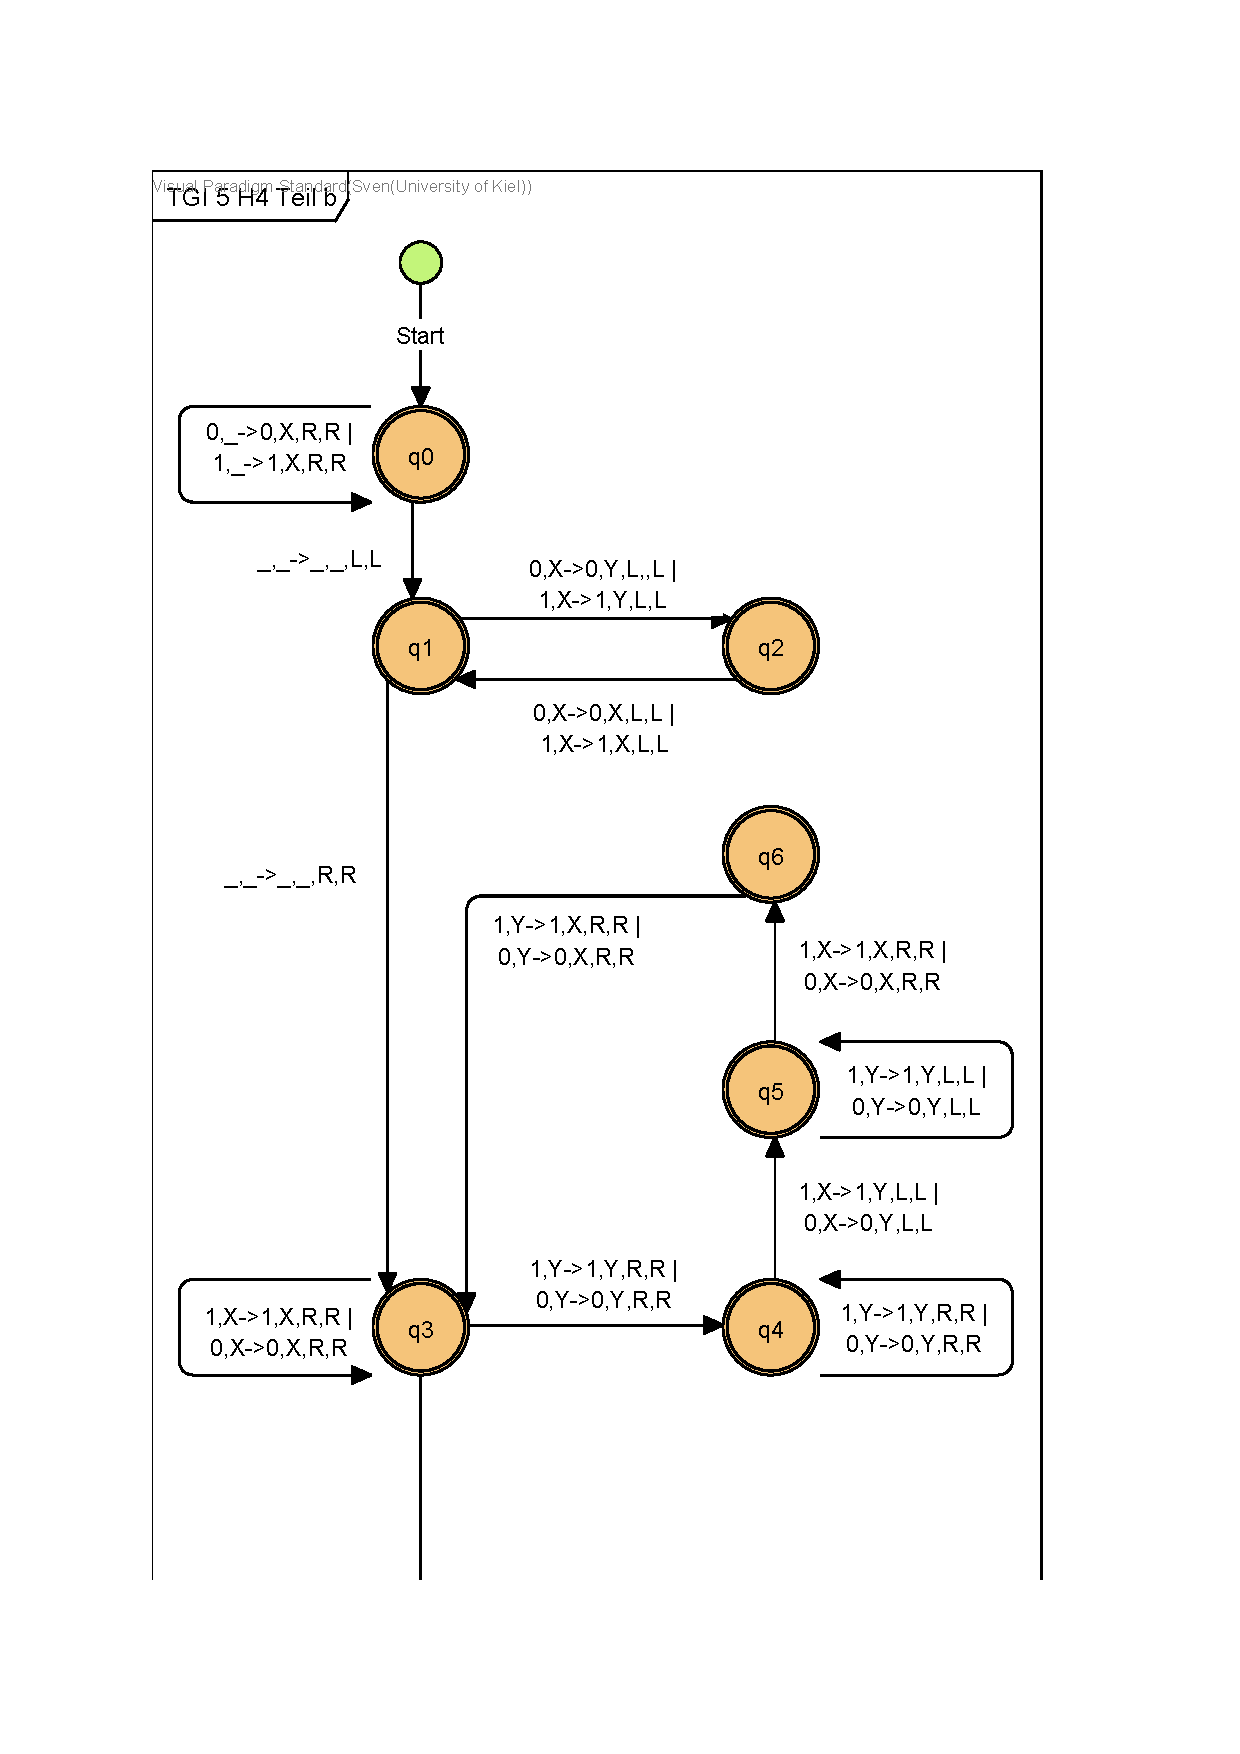
\includepdf[pages=-]{TGI_5_teil_b.pdf}
 

\subsection*{c)}
1. Kopiere Wort bis \# in das 2. Band. \\
2. Addiere 1 zu der Kopie.\\
3. Vergleiche Kopie mit dem zweiten Teil des Wortes. \\
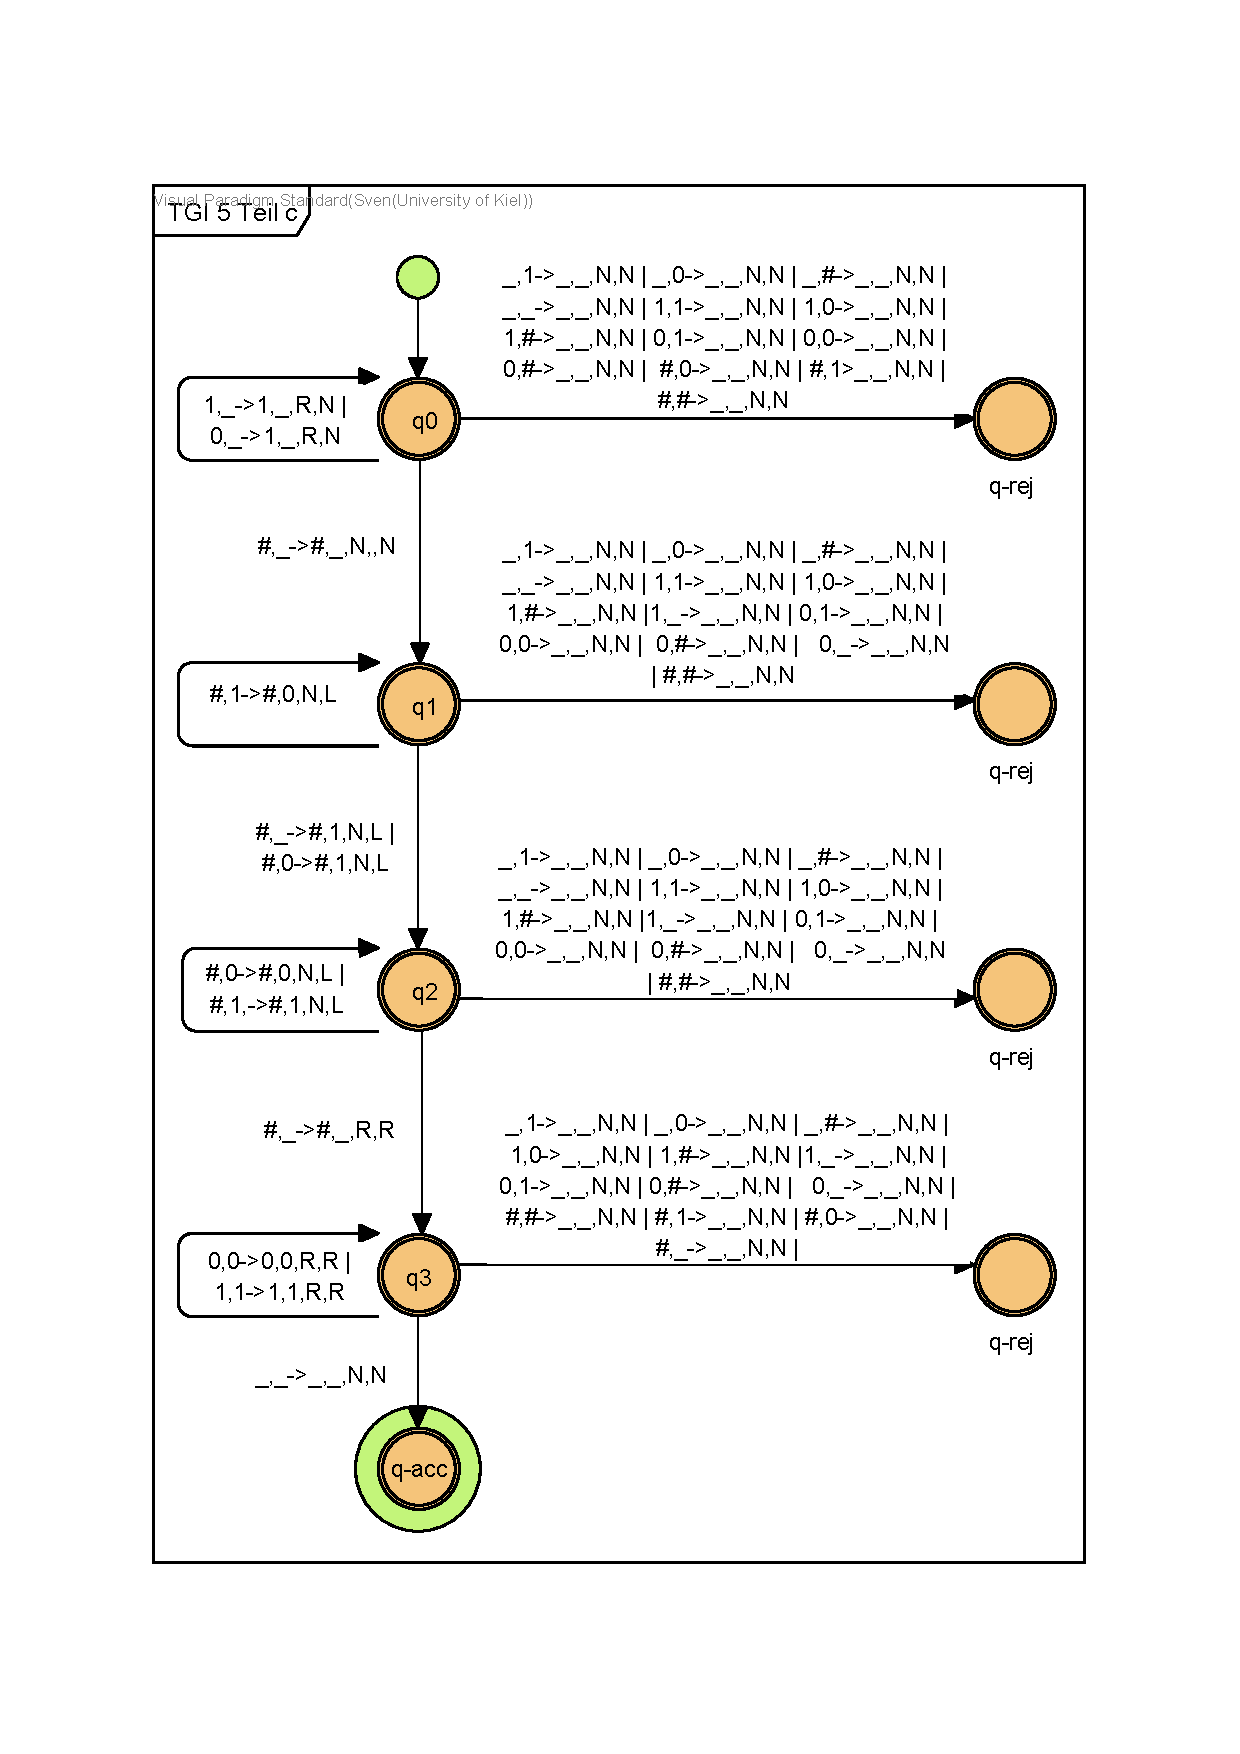
\includepdf[pages=-]{TGI_5_teil_c.pdf}
